%!TEX root = ../Thesis.tex
\chapter{The Aggregator} % (fold)
\label{cha:aggregator}%\marginnote{The original contribution of this chapter is the functional aggregator reference architecture.}
\newchapter{T}{he concept of aggregators} has become widespread in the smart grid literature, yet the concept is still not clearly defined. This leads to a wide range of interpretations of the aggregator concept. This chapter contributes to the field of smart grid by analysing the aggregator through concepts from computer science and system engineering. Specifically, the concept of \emph{functional reference architectures} is applied to the aggregator, making an encompassing definition of what an aggregator is, as well as defining an aggregator lexicon\footnote{In this context, an aggregator lexicon refers to the definition of a vocabulary related to the aggregator concept.}. Furthermore, the candidate functional reference architecture establishes the essential functions aggregators must possess for effective service provision. This contribution is important for harmonizing the understanding of the aggregator, which enables the evaluation and comparison of aggregators. This will by extension ease the integration of aggregators in the power system. Most of the concepts presented here were originally presented as a work-in-progress conference paper\fcite{bondy2015a} which can be found in Appendix~\ref{app:etfa2015}. 

\section{Background}
\newsection{A}{ggregators have been designed} and discussed widely in literature. This section presents the reference framework concept, a taxonomy\footnote{In this context, an aggregator taxonomy refers to a classification of aggregators based upon certain properties.} overview of current aggregator designs, and discusses the concept of flexibility. 
\subsection{The Need for a Reference Architecture} % (fold)
\label{sub:ReferenceArchitecture}
A reference architecture\marginnote{The standard ISO/IEC/IEEE 42010 defines \emph{architecture} as: fundamental concepts or properties of a system in its environment embodied in its elements, relationships, and in the principles of its design and evolution.} ``captures the essence of existing architectures, and the vision of the future needs and evolution to provide guidance to assist in developing new system architectures.''\fcite{cloutier2010concept}. It should provide: 
\begin{itemize}
\item a common lexicon and taxonomy,
\item modularization and the complementary context, and
\item a common (architectural) vision.
\end{itemize} 

This concept is not new in power systems, as can be seen from the draft technical report \emph{IEC 62357-1: Power systems management and associated information exchange -- Part 1: Reference architecture}, which focuses on the mapping of the interactions of all IEC standards related to the interactions of actors, components and systems within the power system. This is done with the aid of the \gls{sgam} which serves as a smart grid reference architecture\fcite{cen2015sgam}. These reference architectures arise due to the need of harmonizing the interactions within smart grids. Similarly, we propose a reference architecture to harmonize the understanding of the capabilities of aggregators. This is needed because:
\begin{itemize}
	\item Existing concepts and methods for benchmarking and generator validation cannot readily be translated from the generator based paradigm to the distributed paradigm of aggregators and flexibility services.
	\item Historically, ancillary services have been defined using a physical understanding of generator capabilities. There is a trend of changing the definitions towards technology-agnostic service models\footnote{As presented in Section~\ref{sec:RedefiningAncillaryServiceRequirements}.}.
	\item Service verification has been done through on-site measurements, which is infeasible with thousands of units participating in service provision.
\end{itemize}

The definition of a reference architecture for aggregators addresses these three issues, and enables benchmarking of aggregator architectures.
Various types of aggregator implementation exist, realizing different design ideas for different sets of requirements. These requirements -- and consequently the designs derived from them -- are unlikely to converge towards a single solution because of the trade-offs involved, e.g. scalability and complexity. A common lexicon and taxonomy is a minimal precondition for aggregator comparison.
If a reference architecture is to be used to describe many of these different designs, it must be highly modular. In practice, the essential functions of the aggregator must be distilled, in order for these functions to be usable as building blocks for the reconstruction of the \emph{particular} functionality of a given implementation. 
The functions are arranged in a reference architecture such that metrics can be assigned to individual functions. In this way, the reference architecture can be used for the documentation of aggregator capabilities, which is part of the prequalification process\footnote{See Chapter~\ref{cha:validation}.}.% Our architectural vision accounts for the need for verifying distributed flexibility services.

% subsection The Need for a Reference Framework (end)
\subsection{Aggregator Taxonomy} % (fold)
\label{sub:Aggregator Taxonomy}
In this work the concept of aggregation encompasses the creation and management of a portfolio of DERs\footnote{DERs can be referred to flexibility resources, or flexibility assets, when they form part of an aggregation portfolio} which seeks to provide the pooled flexibility in power consumption/production as a service or product to the power markets. This general definition covers most uses of the word in literature, but there is a large variation in the functionality that is expected from these aggregators. This can be seen by the wide variety of aggregator designs in literature\footnote{See \eg\cite{kok2005powermatcher,han2010development,sortomme2011optimal,costanzo2013coordination}.}. The main reason for this has been that aggregators have been designed for specific kinds of units, for specific market rules and for specific services. An aggregator taxonomy is helpful for establishing a common understanding of what an aggregator is (and is not) expected to do, and how it is anticipated to perform.

In some works\fcite{fenix2009} a distinction between aggregators is made in terms of which kind of task they perform. If they provide ancillary services they are categorized as Technical \Glspl{vpp} and if they trade energy in the day-ahead energy market they are catalogued as Commercial VPPs. But recent work\fcite{niesse2014conjoint} proposes a \emph{Dynamic VPP}, which is an aggregator that is designed to participate both in day-ahead markets and ancillary service markets. This type of advanced design could become commonplace in the future, making the \emph{Commercial} vs. \emph{Technical VPP} classification obsolete.

Other works classify\fcite{kosek2013overview} aggregators based upon their control paradigm into autonomous, direct, indirect and transactional control. While this classification is more robust towards future aggregator designs, it falls short on one main issue: \emph{where is the intelligence located?}. In other words, the responsibility\footnote{The concept of responsibility is central to the operation of the power system, since it determines which market player is to pay for system imbalances.} and location of decision making is not taken into consideration in this classification. The responsibility and location of the decision making impacts the internal payment settlement of the aggregator, the scalability of the solution, the robustness towards communication faults and the response time, therefore it must be taken into account. In order to do this, a new taxonomy has been proposed\fcite{han2016review}, which identifies six classes of aggregator architectures ranging from fully centralized decision making, passing through diverse forms of distributed decision making, to fully autonomous\footnote{The control paradigm classification can be considered a further sub-classification within this taxonomy.}. Through this taxonomy, it is clear how the architecture of the aggregator will impact the performance in service provision.

% subsection Aggregator Taxonomy (end)
\subsection{The Concept of Flexibility} % (fold)
\label{sub:Flexibility}
Another concept that needs to be defined is the one of \emph{flexibility}. The understanding of the term has evolved over time, but it has been used loosely as the amount of power consumption a unit is able to move in time, within the constraints set by the primary function of the unit, \eg transportation in the case of an EV. The concept of flexibility within the operation of the power system has been discussed in the literature, \eg \emph{F. Sossan}\fcite{sossan2014indirect} presents two types of flexibility: 
\begin{description}
	\item[Type 1:] when customers change their consumption due to changes in prices, \eg with time-of-use tariffs,
	\item[Type 2:] the implicit flexibility in the process of a unit that allows it to change its consumption without affecting its primary function.
\end{description}
It is only \emph{type 2} flexibility that is able to provide verifiable services, and therefore \emph{type 1} flexibility will not be discussed for the rest of this work.

Within the frame of \emph{type 2} flexibility, a taxonomy was proposed by \emph{Petersen et al.}\fcite{petersen2013taxonomy} where flexibility is catalogued as \emph{buckets}, \emph{batteries} and \emph{bakeries}, and in \emph{Hansen et al.}\fcite{hansen2014demand} it is shown how this taxonomy can be applied to a comprehensive set of DR schemes. While this taxonomy covers both the volume of power moved and time the consumption is moved, it is only on the time axis that it considers discrete changes. For example, a \emph{bakery} unit must run for a fixed time, e.g. one hour, and its process can be moved in time but must always run for one hour from the moment it starts, while a \emph{battery} type of unit can stretch or shrink its consumption on the time axis. This means that the taxonomy does not take the power granularity\footnote{Here granularity is meant as the discrete changes in power consumption a flexibility asset is able to realize.} of the flexibility into account. For example, some units can only be controlled through on/off switches and can therefore only provide fixed changes in consumption, while other units are able to provide a range of changes in consumption. Under the current assumption, \ie that flexibility services will be provided by a large amount of small-size units, this limitation of the taxonomy seems irrelevant, since the power change limitation will be smoothed out because of the portfolio aggregations. However, if the volume requirements for services are reduced in the future, thus enabling aggregators with small portfolios, it might be relevant to further expand this flexibility taxonomy. This could, for example, be done by splitting the categories into \emph{continuous} and \emph{discrete} buckets, batteries and bakeries.

Also, two more flexibility concepts must be considered: \emph{deferred} and \emph{curtailed} flexibility. When flexibility is provided as \emph{curtailed} flexibility,  it means that the consumption/generation is reduced/increased without the need to recuperate/shed the energy provided in the service\footnote{The \emph{buckets} in the taxonomy of \emph{Petersen et al.}.}. Correspondingly, \emph{deferred} flexibility is where the units providing the service need to return to a nominal state by recuperating or shedding energy. In demand response, the latter is the most common kind of flexibility used.

In essence, flexibility has two dimensions:
\begin{itemize}
	\item A power (or energy) component, at a given volume and granularity, which the aggregator can offer, and
	\item A time component, which affects:
		\begin{itemize}
			\item the time horizon over which the change in consumption/production can be sustained, and/or
			\item the time granularity of the offered flexibility\footnote{The time and power granularities are important if the service is provided by units whose main process has time constraints, \eg minimum on-time for compressors, and power constraint, \eg only on-off capabilities of the full power rating.}.
		\end{itemize}
\end{itemize}
The quantification of this flexibility is out of the scope of this work, but methods for this are being developed\fcite{bucher2015operational,sossan2014indirect}.

A final observation with respect to flexibility is that system operators like Energinet.dk, the Danish TSO, are interested in acquiring flexibility from aggregators. The traditional approach to buying ancillary services is that the operator pays for an increase or decrease in power production, but flexibility has the extra time dimension. System operators expect flexibility services to fit in within the existing framework, but the two kinds of services can arguably be said to be essentially different. This might lead to undesired consequences such as the kickback effect\footnote{See the aggregator limitations presented in Section~\ref{sec:aggadvantlim}.}. 

% subsection The Concept of Flexibility (end)
\section{Clarifying the Aggregator Concept}
\newsection{R}{esponsibility is a central} concept within power systems. While it is technically possible to provide DR-ancillary services without an aggregator, it is impractical for each DER owner to enter into a contractual agreement for rendering services to the system operators\footnote{The term \emph{system operators} is used throughout this work to refer to both Transmission System Operators and Distribution System Operators.}. In this sense, the aggregator becomes a legal entity that absorbs the legally binding responsibility of its customers and ensures that the aggregated portfolio follows an aggregated operation schedule. At the same time, the aggregator has an ICT infrastructure, which encompasses both the communication and decision making of the aggregator. It uses this infrastructure to coordinate the DERs/flexibility assets' behavior to match a service need of a higher volume than what an individual unit would be able to cover. Also, the aggregator entity will typically not own the flexibility assets it controls. This multi-domain approach to defining aggregators can be seen in Figure~\ref{fig:MAINdomains}.

\begin{figure}[htbp!]
\centering
\includegraphics[width=0.7\textwidth]{domains3.eps}
\caption{The aggregator concept across domains. The aggregator is present in the physical domain with the ICT system, the legal domain through its service contracts, and the control domain through its decision making logic regarding the behavior of the flexibility assets. This figure is an adaptation of Figure~\ref{fig:domains}.}
\label{fig:MAINdomains}
%\vspace*{-5mm}
\end{figure}

These concepts lead to the following definitions:
\begin{description}
	\item[Aggregator role:] The role in the power system of performing aggregation with the purpose of selling the flexibility in consumption or production. The sale of flexibility can be a service to system operators or it can be traded in day ahead markets. The aggregator role can be assigned to a new player in the markets, or it can be assigned to an existing player, \eg a Balance Responsible Party or a utility\footnote{How this role is integrated into the market is still an open question but proposals can be found in \cite{usef2015,heussen2013a}.}.
	\item[Aggregator entity:] The legal entity of the aggregator, which enters into contractual agreements with the other market players and flexibility asset owners. This entity is legally responsible for complying with the contractual agreements.
	\item[Aggregator infrastructure:] The ICT and instrumentation infrastructure, both in terms of software and hardware, that the aggregator owns and operates in order to control the flexibility assets.% \todo{Discuss with Kai and Oliver, I think I'm messing up some terms here}
	\item[Aggregator architecture:] How are the control elements and aggregator functions are related.% \todo{fix this} The shape of the aggregator infrastructure. This encompasses not only the control strategy, but a series of essential functions which will be described in Section~\ref{sec:MAINaggrefarch}.
	\item[Aggregator:] The term used to refer to a market player that has an aggregator role, entity and infrastructure.
\end{description}

Aggregators provide two kinds of services\footnote{The terminology used in Appendices~\ref{app:etfa2015} and \ref{app:isgt2014} varied slightly before settling on the terminology presented in this section.}:
\begin{description}
	\item[Flexibility services] which are provided to system operators and BRPs. These will take the form of ancillary services for the TSO, distribution system services for the DSO and portfolio balancing services for the BRP\footnote{The mentioned types of services will be expanded upon in Chapter~\ref{cha:services}.}.
	\item[Asset management services] provided to the owners of the units, which consists of managing the flexibility asset for the owner, so that it can participate in the flexibility service provision, while still respecting the primary use/comfort settings of the asset owner.
\end{description}
This is shown in Figure~\ref{fig:market_futureMAIN}, where the aggregator is selling services to the TSO through the Consumption BRP and directly to the DSO. This is a market setup which was concluded upon in the iPower project\fcite{hansen2014flechtso}, although this project establishes the Flexibility Clearing House as a mediator between system operators and aggregators\fcite{heussen2013a}. Other market setups allow for the aggregator to participate directly in the market, as long as they coordinate with their corresponding Consumption BRP, such that the aggregator avoids provoking imbalances at the level of the Consumption BRP.
\begin{figure}[htbp!]
\centering
\includegraphics[width=1.0\textwidth]{market_futureMAIN.eps}
\caption{A hypothetical schematic of the aggregator as a service provider. This figure is a modified version of Figures~\ref{fig:marketfuture} and \ref{fig:TSGmarket}.}
\label{fig:market_futureMAIN}
%\vspace*{-5mm}
\end{figure}

Finally, one of the central points of this work is that aggregators are essentially different from traditional generators. Aggregators differ from traditional generators in the sense that\footnote{The differences pointed out here are further expanded upon in Section~\ref{subsec:backgroundvalidation}.}:
\begin{enumerate}
	\item they are distributed systems where each unit has its own response properties, therefore the overall response behaves very differently than that of traditional generators;\label{point:aggblackbox}
	\item they have no single point of measurement, which means the traditional measuring requirements can not be met;
	\item reliability concepts must be adapted to their distributed nature, both in terms of communication reliability and service reliability;
	\item aggregator architectures will vary widely, and each architecture will be sensitive to different operation scenarios;
%	\item while traditional generators follow operational schedules, \ie they have a baseline, aggregators are not required to follow schedules in the same way;
%	\item the primary use of the flexibility assets is to satisfy its owner's need, not to trade power consumption/production in the electricity markets, and it may be that the asset is part of a larger process.
\end{enumerate}

Furthermore, traditional generators follow operational schedules, \ie they have a baseline upon which the service is verified. Estimating the baseline for an aggregator is a difficult\fcite{bode2013incorporating} and may lead to defining alternative methods for service verification.
%While the dynamics of fossil-fueled power plants are well understood and can be modelled based upon physical equations, aggregators can only be analyzed as black boxes.
\section{Advantages and Limitations of Aggregators}\label{sec:aggadvantlim}
\newsection{A}{s stated in the} previous section, the aggregator is a cross-domain entity. Most of the literature on aggregators and demand response focuses on the advances in the control domain which bring \emph{operating}, \emph{planning} and \emph{economic} advantages to the power system\fcite{oconnell2014benefits}. In this work the focus is on the \emph{operating} advantages and limitations introduced by aggregators. 
\subsection*{Advantages}
The operating advantages of aggregators can be divided into three categories: \emph{scalability}, \emph{reliability} and \emph{responsiveness}.

In the control domain,\marginnote{The concepts described in this section are focused on aggregators as service providers, but the same concepts can be applied for aggregators trading in the day-ahead or intra-day markets.} the advantages of contracting an aggregator instead of a large amount of individual small sized units are similar to those of the legal domain. That is, the aggregator in its essence can be regarded as a solution for \emph{scalability} of the smart control of flexible consumption or production. It would be possible for a system operator to directly engage all customers in order to buy services, but the coordination of such large quantities is impractical for the system operators. Thus, the system operators can request fewer services with large volume, and the aggregator will then supply this service with its portfolio of units.

Aggregators providing services through demand response can be more reliable that their traditional counterpart\fcite{kirby2007load,callaway2011a}, \ie large central fossil-fueled generators. A fault in one large generator will have a higher impact on the system than faults in several smaller-sized units. This means aggregators may improve the \emph{reliability} of the power system. Also, DERs have limitations in their capabilities, \eg cycling constraints for compressors, but by aggregating a sufficiently large pool of DERs, system operators will not be exposed to these limitations. A large pool of resources also means that the statistical certainty of the average behavior of the pool will be increased.

Lastly, most DERs have very fast response times, which means that compared to traditional coal-fueled power plants, aggregators are able to provide very fast services. This implies that frequency excursions can be stopped faster and at a higher frequency nadir\fcite{vrettos2015integrating}. This leads to system operators requiring smaller reserves for maintaining  the system security\fcite{makarov2008assessing}.

\subsection*{Limitations}
The main technical limitation of aggregators is that most DERs have as a main objective to satisfy the needs of it's owner, \eg transportation in the case of EVs or heating in the case of HPs. Thus, the aggregator is constrained in its flexibility by the primary function of the DERs. Similarly, selling flexibility through aggregators is optional, so an aggregator must make a compelling business case, or other strong incentives, for the DER owner to participate in the service markets.

Another technical limitation is directly related to the kind of flexibility the aggregator provides. In most cases the aggregator will use \emph{deferred} flexibility, where the units need to recuperate after the service delivery. If all units in the portfolio recuperate at the same time, the consumption spike that ensues may be a larger problem than the one the aggregator was contracted to solve. This is also known as the kick-back effect\fcite{han2014identification}. The problem of saturation can also be associated with this. DERs are usually only able to deliver services on short time horizons (compared to traditional generators) due to the limit size of the units. Once a minimum or maximum state has been reached, the flexibility of the unit disappears. This concept can be represented as a set of saturation curves\fcite{thavlov2015thesis}, where asking for large volumes of power means the units can only deliver for short time periods and vice versa.

A non-technical limitation comes from market regulations. Market rules and ancillary service requirements are defined based on the capabilities of traditional generators. This means that aggregators are expected to behave as traditional generators, when they in essence are something completely different. This means that rules and requirements need to be changed if DER capabilities are to be fully exploited\footnote{This topic is addressed in depth in Chapter~\ref{cha:services}.}.

\section{The Functional Aggregator Reference Architecture}\label{sec:MAINaggrefarch}
\newsection{U}{ntil now, the discussion} on the aggregator has been focused on its role in the power system. In order to further the understanding of what an aggregator is, its functionality must be analyzed. One of the main contributions of the presented research is a \emph{Functional Reference Architecture for Aggregators}. The objective of creating a reference architecture is to address the issue of benchmarking and validation/certification of aggregators\footnote{This topic will be discussed in depth in Chapter~\ref{cha:validation}.}. The traditional approach to the certification of generators can not be applied to aggregators, and therefore new methods must be designed. Part of this method is to verify that an aggregator possesses the essential functionality for effective service provision. This essential functionality is defined in the proposed reference architecture.

In order to formulate the aggregator reference architecture, a set of existing commercial and academic aggregators\footnote{The analyzed aggregators were: Open Energi\cite{openenergi}, PowerHub by DONG Energy\cite{powerhub}, the Heterogenous Aggregator by Aalborg University\cite{rahnama2014evaluation} and the D-EMPC\cite{costanzo2013coordination}.}  were deconstructed into their basic functionality. The resulting functions of each aggregator were compared and clustered. From these clusters, a set of generic functions were formulated. The resulting functions are\footnote{For detailed explanations of each function see Section~\ref{sec:funcdec}.}:

\begin{enumerate}[label=\Alph*]
		% external interface
	\item Service Interface: The function that translates information from the legal domain to the control domain\footnote{See Figure~\ref{fig:MAINdomains}.}
		% Monitoring & Supervision modules
	\item Performance Monitoring: The function that evaluates and verifies the behavior of the client unit.
	\item Supervision and Resource Handling: The function that determines the availability and composition of the resource portfolio based upon the performance of the units.
	\item Operator Interface: The function that supports operator decision making.
		% Control related
	\item Control: The function that generates the appropriate control domain signals to manipulate the portfolio behavior.
	\item Flexibility Monitoring: The function that assesses the amount of flexible consumption/production available in the portfolio.
		% Communication
	\item Aggregator-internal Communication: The function that covers the internal communication within the distributed elements of the aggregator.
	\item Client Management: The function that determines the availability of the flexibility assets depending on their communication status.
	\item External Information Services: The function that pulls the necessary external data for the functioning of the aggregator, \eg weather and price forecasts.
	\item Asset Interface: The function that translates between the control domain signals and the specific protocols used by the flexibility asset.
		% The odd one out
	\item Internal-information exchange: The function that enables the exchange of data and other information between the relevant functions of the aggregator.
\end{enumerate}

These generic functions, with exception of \emph{External Information Services}, are present in all aggregators. This exception is found in the cases where the aggregator delivers services based measurements of the grid, \eg Frequency Containment Reserve\footnote{See Chapter~\ref{cha:services}.}. The implementation of each function varies widely. 
Conceptually, each function has a specific purpose and task, but in the actual software implementation of the aggregator, one or more of these functions may be executed in the same module, or may be executed manually by an operator.

The functions can be classified in two different ways: a task based classification and a data-handling based classification. The task based classification divides the functions according to the kind of task the function executes:
\begin{description}
	\item[External interface:] The functions that provide information exchange with entities outside the aggregator infrastructure.
		\begin{itemize}
			\item Service Interface: Outputs a service model that sets the objective of the aggregator.
			\item Asset Interface\footnote{The asset interface may also be considered part of the communication related functions, since it provides the communication translation between the flexibility asset and the rest of the aggregator infrastructure.}: Outputs the DER/flexibility asset data to the rest of the aggregator.
		\end{itemize}
	\item[Monitoring \& Supervision:] The functions that parse information related to the unit portfolio.
		\begin{itemize}
			\item Performance Monitoring: Outputs the performance of the individual and aggregated flexibility assets. Can be used for internal purposes and/or service settlement purposes.
			\item Supervision and Resource Handling: Outputs the portfolio that is available for control, based upon the performance/compliance of the units.
			\item Operator Interface: Outputs manual decisions with respect to the portfolio and control.
		\end{itemize}
	\item[Control related functions:] The functions that involve the automated decision making with regards to the unit behavior manipulation.
		\begin{itemize}
			\item Control: Outputs control domain signals, \eg activation or reference signals to the flexibility assets. This is highly dependent on the specific control architecture that the aggregator implements.
			\item Flexibility Monitoring: Outputs the state of the DERs/flexibility assets in terms of the flexibility available for control.
		\end{itemize}
	\item[Communication:] The functions that relate to the internal communication of the aggregator.
		\begin{itemize}
			\item Aggregator-internal Communication: Passes information
			\item Client Management: Outputs the portfolio of connected and responsive units.
			\item External Information Services\footnote{Since the external information services only pull information from outside of the aggregator, and no information exchange is carried out, this function is not considered part of the external interface functions.}: Outputs the required external data.
		\end{itemize}
	\item[Knowlegde exchange:] This category only covers the Internal-information Exchange. It enables the information exchange between all parts of the aggregator. It can take any form, from a simple bus to highly developed data storage system, and has no specific output by itself.
\end{description}
This classification is represented in Figure~\ref{fig:MAINrefarch} through the symbols marked on each function block.

The data-handling based classification is done by grouping the functions based on how data/information is handled in the function. This classification is reflected in Figure~\ref{fig:MAINrefarch} through the color code. The function classes are the following:
\begin{description}
	\item[Enabler functions:] Those functions that only pass the data/information on to other functions.
	\item[Information interpreters:] Those functions that convert data into information.
	\item[Decision making functions:] Those functions that use the information to make decisions.
\end{description}

The functions defined here abstract from any specific implementation of an aggregator\footnote[][-2cm]{Usually, a reference architecture must also define the relationship between its functions, but in this case, arrows representing data flow were avoided in the design, since they presuppose a specific aggregator architecture}, and provide the building blocks for the functional reference architecture shown in Figure~\ref{fig:MAINrefarch}\footnote{This diagram is a correction of the one presented in Appendix~\ref{app:etfa2015}.}. This figure is a description of what the \emph{aggregator infrastructure} block from Figure~\ref{fig:MAINdomains} encapsulates.
\begin{figure}[htbp!]
\centering
\includegraphics[width=1.0\textwidth]{diag_simple3.eps}
\caption{A visual representation of the proposed reference architecture. The symbols represent data types that are outputs to the functions, and the color represents the data-handling categorization of the functions.}
\label{fig:MAINrefarch}
\end{figure}
Although the reference architecture abstracts from specific implementation, we present below an example of how an aggregator can be mapped to the reference architecture.
\subsection{Application Example: Open Energi}
As an example, the aggregator architecture for the British company Open Energi is described using the reference architecture. The information on how their aggregator functions was acquired through a publication\fcite{cheng2014availability} and unofficial email-interview with one of their developers.

Part of Open Energi's business model is to provide frequency response to National Grid, the TSO of the United Kingdom, by controlling the heating of bitumen tanks. This is achieved by installing a unit on each bitumen tank that can react upon changes in the grid frequency. How the control algorithm coordinates all units for an appropriate response is a company secret, but we were given enough information\footnote[][-2em]{Note that Open Energi has not had the opportunity to review this example, and can therefore not be taken as an accurate example.} to describe Open Energi with the reference architecture as presented in Figure~\ref{fig:openenergirefarch}.

\begin{figure}[htb]
\centering
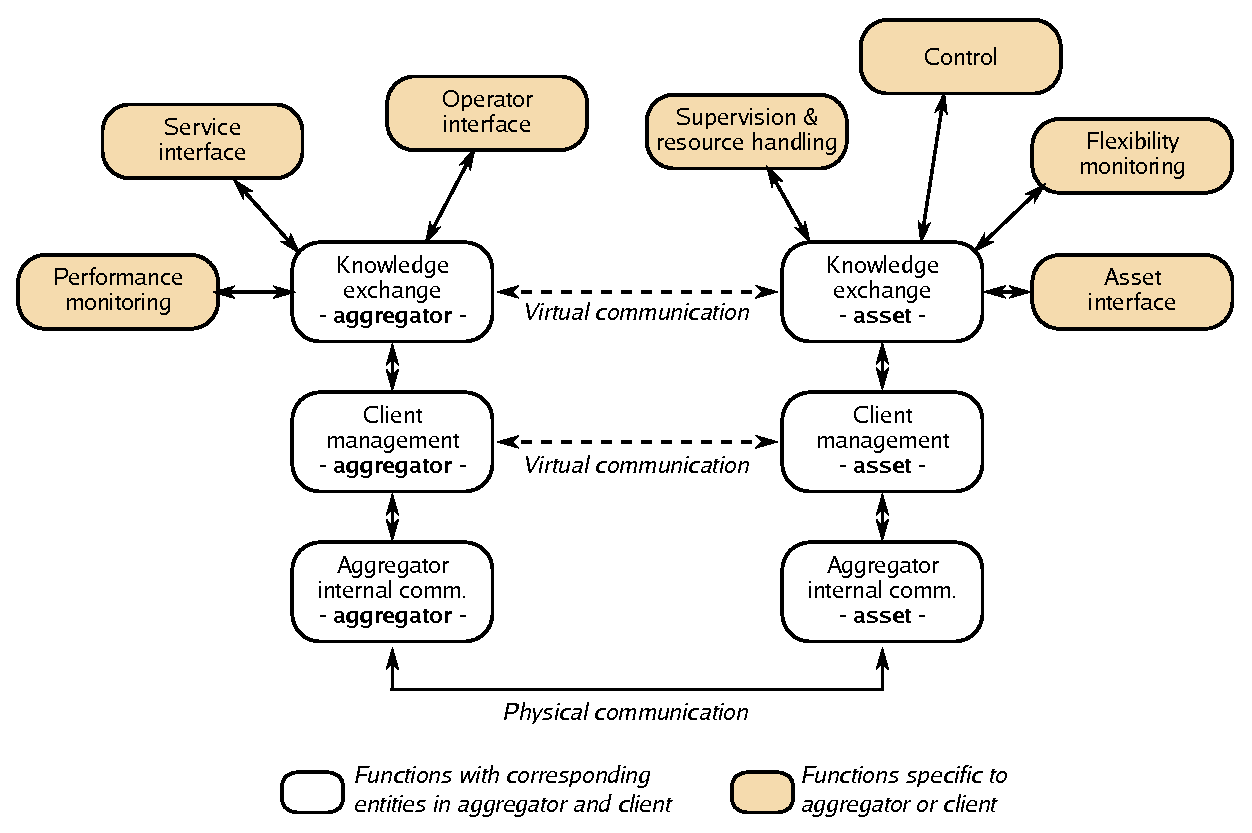
\includegraphics[width=1.0\textwidth]{stackdrawing_openenergi.eps}
\caption{Mapping the Open Energi aggregator to the functional reference architecture. In this case it is only blocks related to communication that appear both at the aggregator and asset side.}
\label{fig:openenergirefarch}
\end{figure}

In this case autonomous, fully-distributed architecture is represented by having  most of the \emph{decision making} and \emph{information interpreter} functions on the asset side, and only having the operator interface, portfolio performance assessment and service interface on the aggregator side. When this mapping is complete, it can be used as documentation for the compliance of the aggregator with the reference architecture, which can serve as the documentation step of the prequalification process\footnote{See Chapter~\ref{cha:validation}.}.

\section{Conclusions Regarding Aggregators}
\newsection{T}{he concept of aggregators} is widespread in the smart grid literature, but the interpretations of what an aggregator is varies widely. One of the contributions presented in this chapter is to provide a common lexicon and reference architecture for aggregators so that discussion on the topic can be harmonized. This will hopefully lead to faster advances in the field. Also, the functional reference architecture is to be used in aggregator validation and certification\footnote{The concept of aggregator validation and certification is discussed in depth in Section~\ref{sec:aggpreq}, where it is also discussed how this functional reference architecture can be useful.}. A secondary use for the reference architecture is to serve as a guide for future designs of aggregators.

When aggregators are discussed in the academic literature, the focus is usually on the control function. The functional reference architecture makes it clear that aggregators are more complex than single control block. There are several implicit functionalities, \eg the \emph{enabler functions} that are glossed over in academic studies, but are important for understanding the full capabilities the aggregator.

A current shortcoming of this work is that the presented functional reference architecture for aggregators is part of a work-in-progress paper and as such, needs to be refined and extended. Future work will include the design of key performance indices assigned to each function, such that the scores can be used to gain a better understanding of the capabilities of the aggregator and evaluate the maturity of the aggregator. 

% chapter The Aggregator (end)
